\documentclass{article}
% packages
\usepackage{gensymb}
\usepackage{amsmath}
\usepackage{graphicx}

% smaller page margins
\usepackage[top=2in, bottom=1.5in, left=1.5in, right=2in]{geometry}

% inline TODO: notes
\usepackage[textwidth=1.75in]{todonotes}

% for \FloatBarrier
\usepackage{placeins}

% graphics setup
\DeclareGraphicsExtensions{.eps,.pdf,.png,.jpg}

\begin{document}
\section{Block diagram}
soon

\section{Inputs and outputs}
	\subsection{Inputs}
	\begin{tabular}{ l | l | l  }
		Input					&	Symbol		&	Unit		\\	\hline
		DC current			&	$I_{dc}$		&	A		\\
		Ambient temperature	&	$T_{amb}$	&	\degree C \\ 
	\end{tabular}
	
	\subsection{Outputs}
	\begin{tabular}{ l | l | l  }
		Output					&	Symbol		&	Unit		\\	\hline
		Internal charge				&	$Q$			&	coulomb	\\
		Terminal voltage			&	$V_{dc}$		&	V		\\
		Internal temperature			&	$T_{pack}$	&	\degree C	\\
	\end{tabular}
	
\section{Background, rationale, modeling strategy}
	\subsection{Electrical model}
		Each battery cell is modeled as an equivalent circuit:
		
		\begin{figure}[h!]
				\centering
				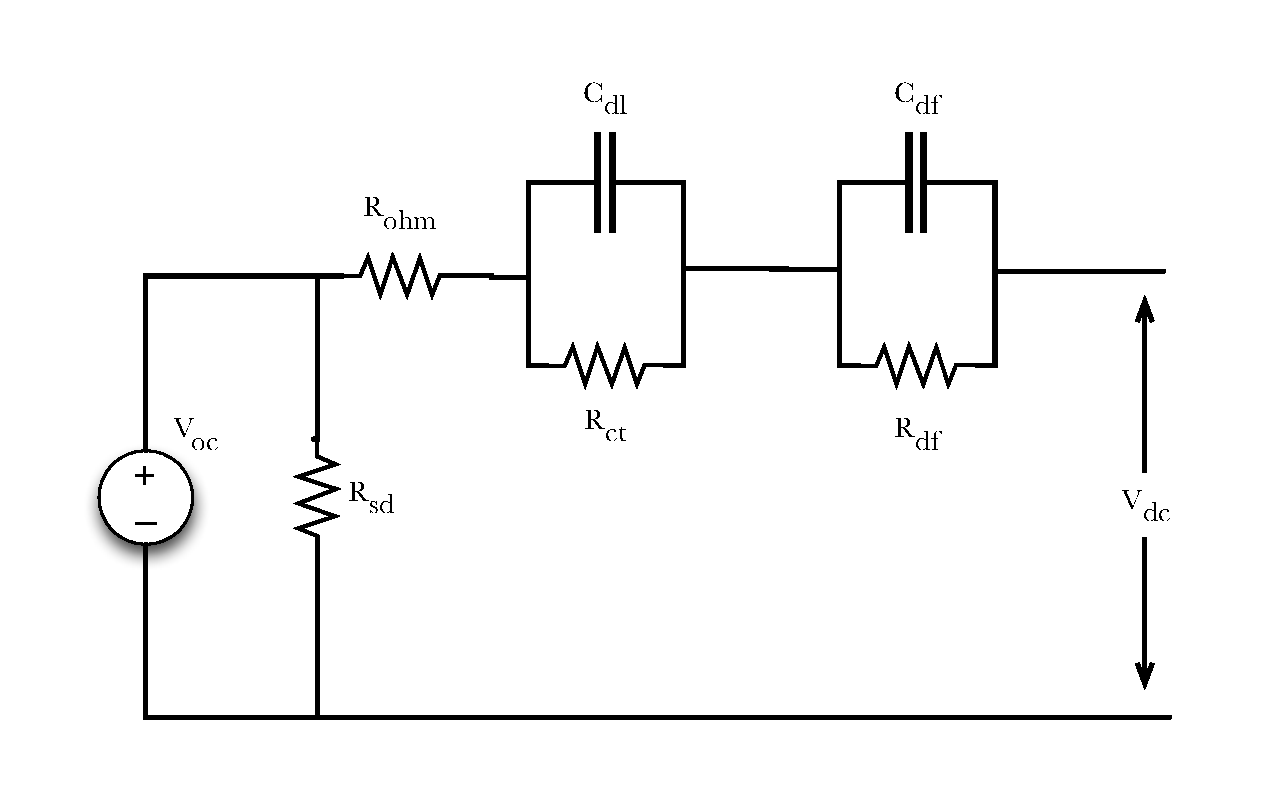
\includegraphics[width=4in]{Figures/Battery_pack_equivalent_circuit}
				\caption{Battery cell equivalent circuit}
				\label{fig:battery_pack_equivalent_circuit}
		\end{figure}
		\FloatBarrier
		
		where:
		\todo{What in Sam Hill do these parameters depend on?}
		\begin{center}
		\begin{tabular}{l l}
			$V_{oc}$		&	is the battery open-circuit voltage in volts	\\
			$R_{sd}$		&	is the battery self-discharge resistance in ohms \\
			$R_{ohm}	$	&	is the battery ohmic resistance in ohms \\
			$R_{ct}$		& 	is the battery ?? resistance in ohms \\
			$R_{df}$		&	is the battery ?? resistance in ohms \\
			$C_{dl}$		&	is the battery ?? capacitance in farads \\
			$C_{df}$		& 	is the battery ?? capacitance in farads
		\end{tabular}
		\end{center}
		
		The battery open-circuit voltage, $V_{oc}$, is a function of the remaining cell capacity Q, and is represented by a lookup table.
		\todo{$V_{oc}$ probably has a temperature dependence as well}
		
		
		\todo{Need to expand this electrical model to the n-series-cell equivalent circuit (assume all cells are identical?)}
		
	\subsection{Thermal model}
		The battery pack is modeled as a single thermal mass which has some thermal resistance to ambient temperature:
		
		\begin{figure}[h!]
				\centering
				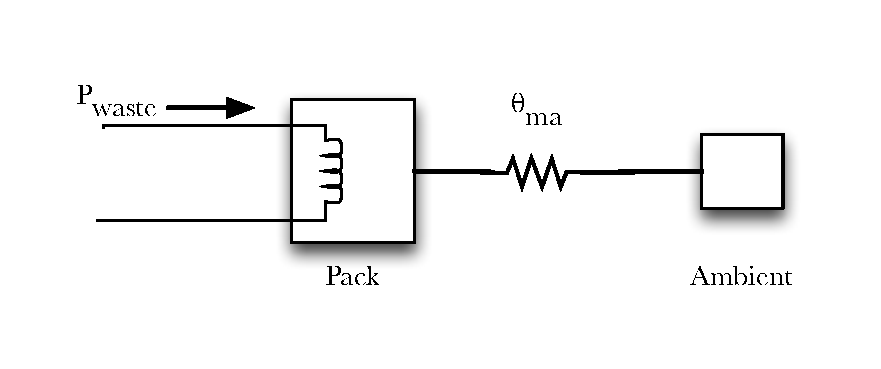
\includegraphics[width=\linewidth]{Figures/Battery_pack_thermal_equivalent_circuit}
				\caption{Battery cell thermal equivalent circuit}
				\label{fig:Battery_pack_thermal_equivalent_circuit}
		\end{figure}
		\FloatBarrier
		
		The waste power (heat input) $P_{waste}$ is the sum of the heat dissipated in each resistance:
		
		\begin{equation}
			P_{waste} = I_{dc} (R_{ohm})^2 + I_{Rct} (R_{ct})^2 + I_{Rdf} (R_{df})^2 + I_{sd} (R_{sd})^2
		\end{equation}
		
		and the thermal resistance to ambient, $\theta_{ma}$, is an arbitrary nonlinear function of vehicle speed, represented by a 1D lookup table:
		
		\begin{equation}
			\theta_{ma} = h(v)
		\end{equation}
		
		where $v$ is the vehicle's longitudinal velocity.
		
		

\section{Parameters}
	\begin{tabular}{ l | l | l  }
		Parameter				&	Symbol		&	Unit					\\	\hline
		Pack thermal mass			&	$C_{th}$		&	$J \text{ \degree C}^{-1}$
	\end{tabular}
	
	\todo{There are more parameters.}



\section{Assumptions}

\end{document}